\documentclass[final]{beamer}

% Packages
\usepackage[scale=1.24]{beamerposter}
\usepackage{graphicx}
\usepackage{booktabs}
\usepackage{amssymb}
\usepackage{amsmath}
%\usepackage{minted}
\usepackage{listings}
\usepackage{xcolor}
\usepackage{tikz}

\definecolor{darkgreen}{rgb}{0,0.6,0}
\lstdefinestyle{Python}{
    language        = Python,
    basicstyle      = \ttfamily,
    keywordstyle    = \color{blue},
    keywordstyle    = [2] \color{teal}, % just to check that it works
    stringstyle     = \color{green},
    commentstyle    = \color{darkgreen}\ttfamily
}

% Styling
\newcommand{\agsNote}[1]{\textcolor{cyan}{#1}}
\newcommand{\bfCenter}[1]{\centerline{\textbf{#1}}}
\usetheme{confposter}
\setbeamercolor{block title}{fg=blue,bg=white}
\setbeamercolor{title}{fg=red,bg=white}
\setbeamercolor{block body}{fg=black,bg=white}
\setbeamercolor{block alerted title}{fg=white,bg=blue}
\setbeamercolor{block alerted body}{fg=black,bg=white}

% Formatting
\newlength{\sepwid}
\newlength{\onecolwid}
\newlength{\twocolwid}
\newlength{\threecolwid}
\setlength{\paperwidth}{48in}
\setlength{\paperheight}{36in}
\setlength{\sepwid}{0.024\paperwidth}
\setlength{\onecolwid}{0.22\paperwidth}
\setlength{\twocolwid}{0.464\paperwidth}
\setlength{\threecolwid}{0.708\paperwidth}
\setlength{\topmargin}{-1in}

\newcommand{\dif}{\mathrm{d}}

% Meta Data
\title{Community Supported Quasi-Monte Carlo (QMC) Software}
\author{ Fred Hickernell (\texttt{hickernell@iit.edu}), Sou-Cheng Choi (\texttt{schoi32@iit.edu}), Aleksei Sorokin (\texttt{asorokin@hawk.iit.edu})}
\institute{Department of Applied Mathematics, Illinois Institute of Technology\vspace{-2ex}}

\begin{document}
% logos
\addtobeamertemplate{headline}{} 
{
	\begin{tikzpicture}[remember picture,overlay] 
	\node [anchor=north west, inner sep=1.5cm] at (current page.north west) {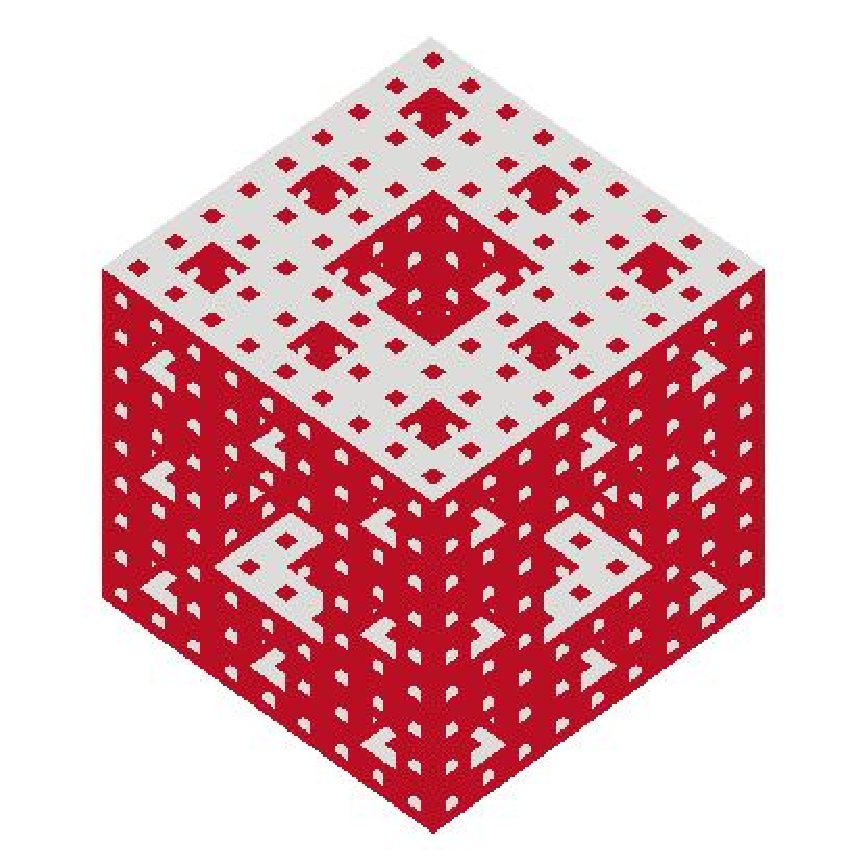
\includegraphics[height=9.5cm]{images/MengerIITRedGray.eps}}; 
	\end{tikzpicture} 
}

\addtobeamertemplate{headline}{} 
{
	\begin{tikzpicture}[remember picture,overlay] 
	\node [anchor=north east, inner sep=1.5cm] at (current page.north east) {
\includegraphics[height=9cm]{images/iit_high_res.png}}; 
	\end{tikzpicture} 
}

% Setup Format and Styling
\addtobeamertemplate{block end}{}{\vspace*{2ex}}
\addtobeamertemplate{block alerted end}{}{\vspace*{2ex}}
\setlength{\belowcaptionskip}{2ex}
\setlength\belowdisplayshortskip{2ex}
\begin{frame}[t]
\vspace{-2ex}
\begin{columns}[t]

% Column 1
\begin{column}{\sepwid}\end{column}
\begin{column}{\threecolwid}
\begin{columns}[t,totalwidth=\threecolwid]  

%    Software Objectives
\begin{column}{\onecolwid}\vspace{-1in}
\begin{block}{Software Objectives}
    To provide QMC software that is: 
    \begin{itemize}
        \item comprised of free open source tools
        \item designed for development and support 
        \item easy to use for non-experts
        \item a recognized standard
    \end{itemize}
\end{block}

%    The QMC Problem
\vspace{-2ex}
\begin{block}{The QMC Problem}

    \bfCenter{Original Form} 
        \begin{equation*}
            \mu = \int_{T} g(t) \, \lambda(\dif t) 
            \label{eq:ogProblem}
        \end{equation*}
        $ g:T \rightarrow \mathbb{R} = $ original integrand \\
        $ \lambda = $ original measure

    \vspace{2ex}
    \bfCenter{Convenient Form}
        \begin{equation*}
            \mu = \int_{X} f(x)\rho(x)dx = \int_{X} f(x) \, \nu( \dif x)
            \label{convForm}
        \end{equation*}
        $\nu = $ well defined probability measure\\
        $\phi: X \rightarrow T = $ change of variables\\
        $f: X \rightarrow \mathbb{R} $ = integrand after change of variables
        
    \vspace{2ex}
    \bfCenter{(quasi-)Monte Carlo Approximation}
        \begin{equation*}
            \hat{\mu}_n = a_n \sum_{i=1}^{n} f(x_i)w_i =  \int_{X} f(x) \, \hat{\nu}( \dif x)
            \label{qmcApprox}
        \end{equation*}
        \begin{align*}
            \nu \approx \hat{\nu}_n & = a_n \sum_{i=1}^n w_i \delta_{\hat{x_i}}(\cdot) \\
            & = \text{discrete probability measure}
        \end{align*}
\end{block}
\end{column}


%    Integrate
\begin{column}{\onecolwid}
\setbeamercolor{block alerted title}{fg=black,bg=red!10}
\begin{alertblock}{Integrate}
    Find $\hat{\mu}_n$ such that $\left | \mu - \hat{\mu} \right  | \leq \epsilon$ \\[1ex]~\
    \textbf{Arguments}
    \begin{itemize}
        \item Function instance
        \item Measure instance
        \item Discrete Distribution instance
        \item Stopping Criterion instance
    \end{itemize}
\end{alertblock}

%    Function
\setbeamercolor{block alerted title}{fg=black,bg=green!10}
\begin{alertblock}{Function}
    Specify and generate values $f(\hat{x})$ for $\hat{x} \in \hat{\nu}$ \\[1ex]~\
    \textbf{Concrete Classes}
    \begin{itemize}
        \item Keister
        \item Asian Call
    \end{itemize}
\end{alertblock}

%    Discrete Distribution
\begin{alertblock}{Discrete Distribution}
    Specify and generate $a_n \sum_{i=1}^n w_i \delta_{\hat{x_i}}(\cdot)$ \\[1ex]~\
    \textbf{Concrete Classes}
    \begin{itemize}
        \item IID
        \item QMC
    \end{itemize}
\end{alertblock}
\end{column} 

%    Stopping Criterion
\begin{column}{\onecolwid}%\vspace{-1in}
\setbeamercolor{block alerted title}{fg=black,bg=green!10}
\begin{alertblock}{Stopping Criterion}
    Determine $n$ \\[1ex]~\
    \textbf{Concrete Classes}
    \begin{itemize}
        \item Central Limit Theorem (IID)
        \item Mean Variance (Mesh)
    \end{itemize}
\end{alertblock}

%    Measure
\begin{alertblock}{Measure}
    Specify components of a general sampling method \\[1ex]~\
    \textbf{Implemented Functions}
    \begin{itemize}
        \item Standard Uniform
        \item Standard Gaussian
        \item IID Zero Mean Gaussian
        \item Brownian Motion 
        \item Lattice base 2
        \item Sobol base 2
    \end{itemize}
\end{alertblock}

%    Accumulate Data
\begin{alertblock}{Accumulate Data}
    Accumulated data required in the computation of the integral
\end{alertblock}
\end{column}
\end{columns}

% Python Example
\begin{column}{\threecolwid}\vspace{-.8in}
\begin{block}{Python Examples}
    \begin{column}{\onecolwid}
        %\inputminted{python}{Keister.snip.py}
        \lstinputlisting[style=Python]{Keister.snip.py}
    \end{column}
    \begin{column}{\twocolwid}
    \vspace{-2ex}
        \begin{figure}
            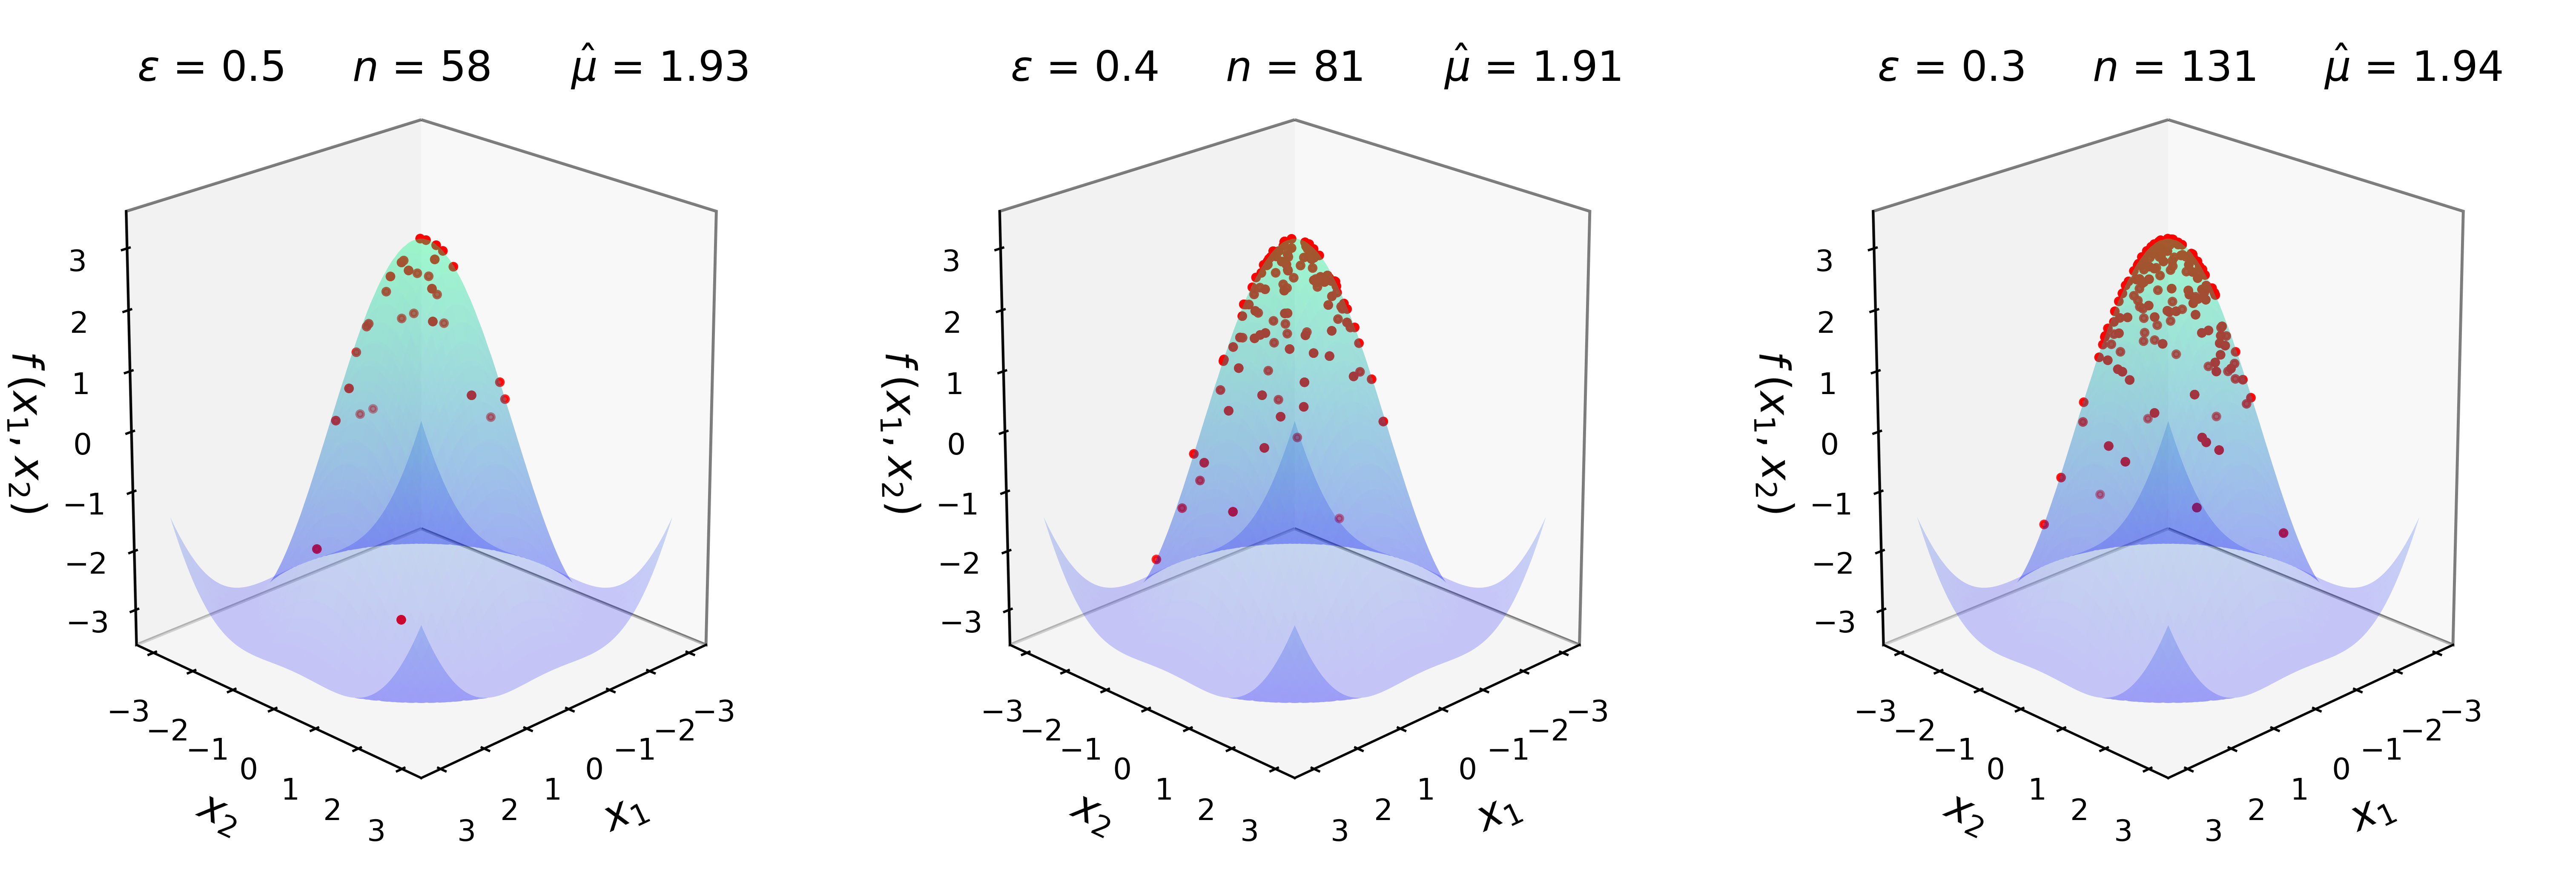
\includegraphics[width=0.96\textwidth]{Images/Three_3d_SurfaceScatters.png}
            \caption{\ Reducing tolerance resulting in more samples and better approximations of the Keister integrand.}
        \end{figure}
    \end{column}
\end{block}
\end{column}
\end{column}

% Results
\begin{column}{\sepwid}\end{column}
\begin{column}{\onecolwid}\vspace{-.3in}
\begin{block}{Results}
    \bfCenter{Integration Time Comparison}
    \begin{figure}
        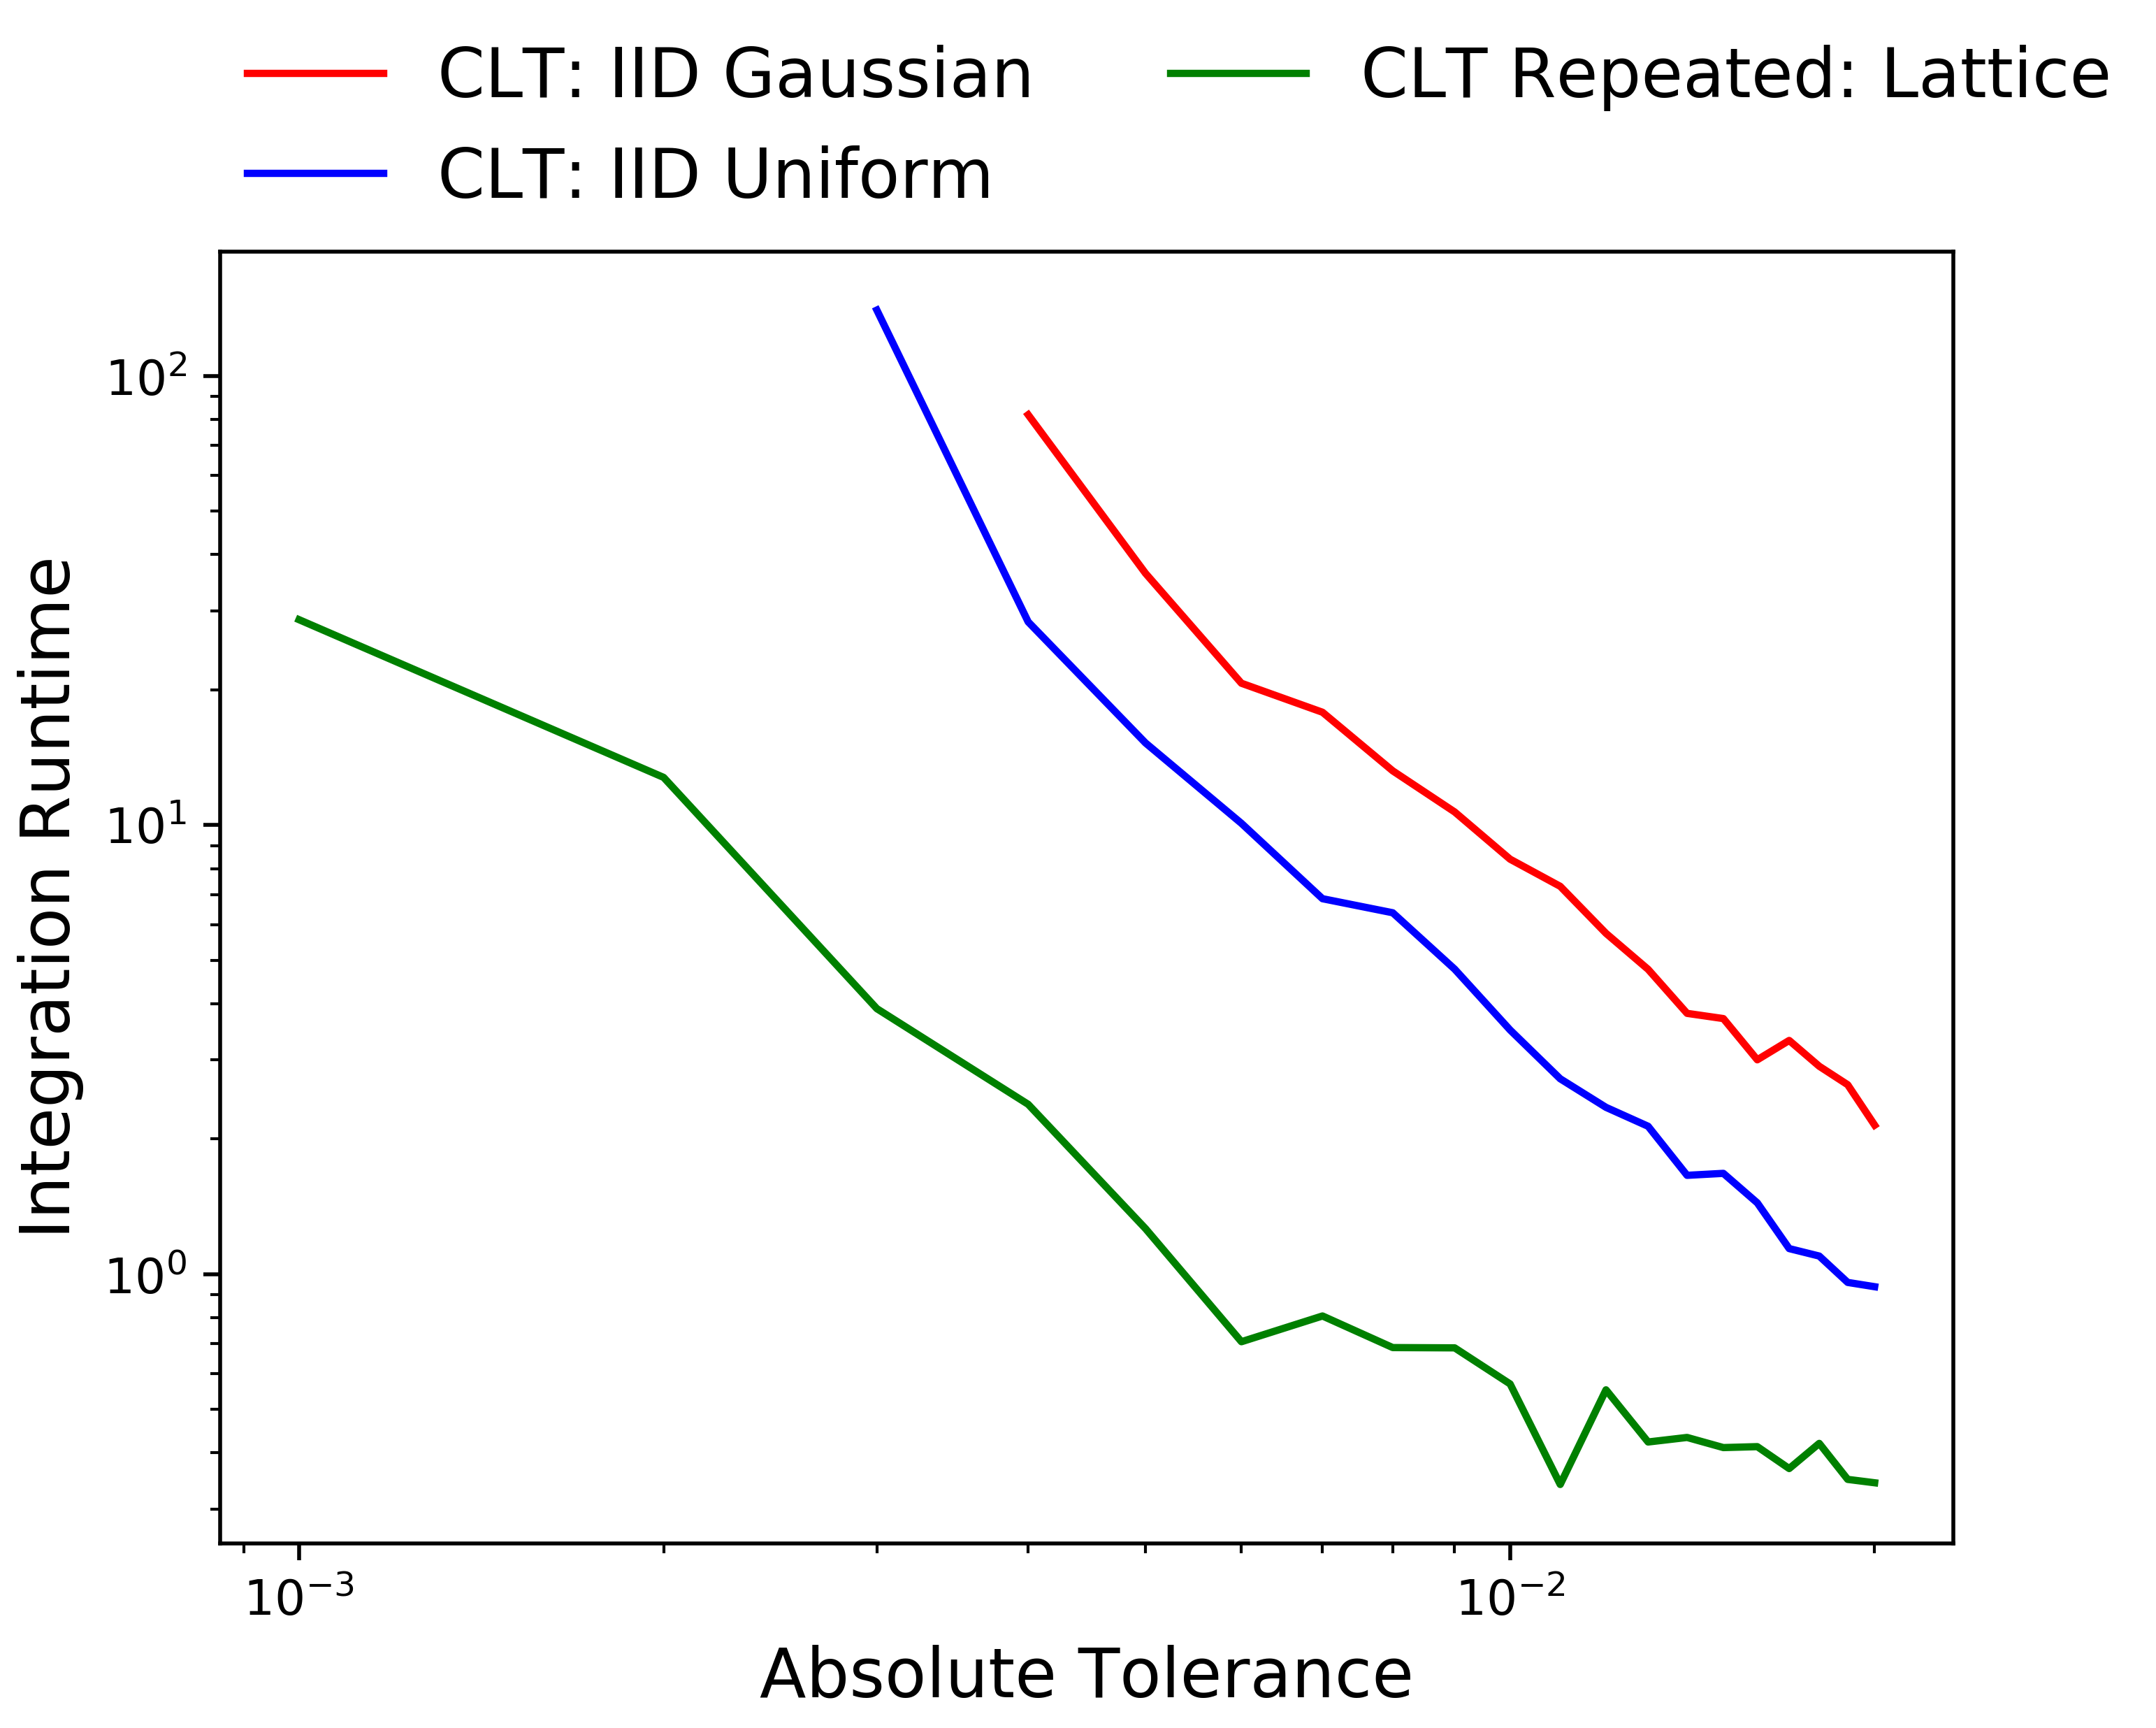
\includegraphics[width=1\textwidth]{Images/AbsTol_Runtime_LinePlot.png}
        \caption{\ Multi-dimensional Asian Call Option integrated with respect to  Brownian Motion.}
    \end{figure}
\end{block}

%    Future Work 
\vspace{-.5in}
\begin{block}{Future Work}
    \begin{itemize}
        \item Enhance tests and examples 
        \item Refine existing components
        \item Expand community of contributors
    \end{itemize}
\end{block}

% References
\begin{block}{References}
\begin{enumerate}
    
    \item Hickernell, Choi, and Sorokin. \textit{QMC Community Software}, MATLAB and Python software, 2019. \textit{Working}. Available at \url{https://github.com/QMCSoftware/QMCSoftware}.
    
    \item Choi,  Ding,  Hickernell,  et al., \textit{GAIL: Guaranteed Automatic Integration Library} (versions 1.0--2.3),
    MATLAB software, 2013--2019. Available at \url{http://gailgithub.github.io/GAIL_Dev/}.
    
    \item Kuo and Nuyens. Application of quasi-Monte Carlo methods to elliptic PDEs with random diffusion coefficients: a survey of analysis and implementation, \textit{Foundations of Computational Mathematics}, 16(6):1631--1696, 2016.

\end{enumerate}
\end{block}
% Acknowledgements
\begin{block}{Acknowledgements}
    Thank you to Dirk Nuyens for providing the lattice and Sobol generators 
\end{block}
\end{column}
\end{columns}
\end{frame}
\end{document}
